\chapter{Mitigate Fingerprinting of Honeypots}
\label{chap:fingerprinting}

\section{Fingerprinting Cowrie}

Attackers have a strong motivation to reveal honeypots before launching an attack.
Without any protection attackers would disclose their methods, and thus, newly developed attacks would become useless.
As shown in \autoref{chap:cloud-security}, attackers do try to get information about the host system.
\citet{vetterl2020} discussed various methods of fingerprinting, however, executing commands in a login shell and examining the response leaves precarious information to the honeypot itself.
In his work he evaluated methods to detect honeypots at the transport level.
As stated, the value of a honeypot would be merely zero if a detection on transport level would work.
He presents fingerprinting methods for SSH, Telnet, and HTTP/Web.
Due to the complexity of each method, we focus on SSH fingerprinting with the honeypot Cowrie.
The idea to detect SSH honeypots is to look for deviations in the response.
Therefore, \citet{vetterl2020} sends a set of probes $P = \{P_1, P_2, \dots, P_n\}$ to a given set of implementations of a network protocol $I = \{I_1, I_2, \dots, I_n\}$ and stores the set of responses $R = \{R_1, R_2, \dots, R_n\}$.
For the given set of responses he calculated the cosine similarity coefficient $C$.
Goal is to find the best $P_i$ where the sum of $C$ is the lowest.
\autoref{fig:draft-cosine-similarity} presents these steps.

Cosine similarity outputs the similarity between vectors of numerical attributes.
In text semantics it is widely used to measure the similarity of sets of information such as two sentences.
\citet{vetterl2020} outlines that it can be used in \enquote{traffic analysis to find abnormalities and to measure domain similarity}.
Mathematically, it computes the angle between two vectors.
For each set of information $A$, we create a vector $D_A$.
Referring to our use case with SSH, we use the response from the server as information $A$.
If $\theta$ is the angle between $D_A$ and $D_B$, then:

\begin{equation} \label{eq:cosine-similarity}
    \cos \theta = \frac{D_A \cdot D_B}{\|D_A\| \|D_B\|}
\end{equation}

where \enquote{$\cdot$} is the dot product obtained by:

\begin{equation}
    D_A \cdot D_B = \sum_{i=1}^{n} (D_{A_i} \times D_{B_i})
\end{equation}

and $\|D_A\|$ (resp. $\|D_B\|$) is the Euclidean norm, obtained by $\sqrt{\sum_{i=1}^{n} D_{A_i}^2}$ (resp. $\sqrt{\sum_{i=1}^{n} D_{B_i}^2}$).
The values of vectors are non-negative. The similarity between items is the value $\cos \theta$, $\cos \theta = 1$ indicates equality.

\begin{figure}[ht]
    \centering
    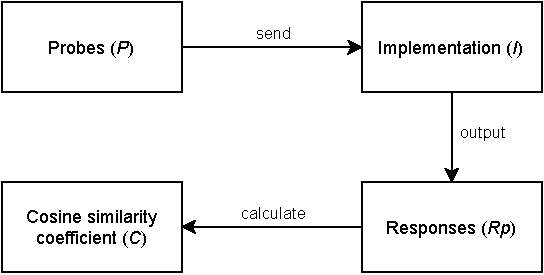
\includegraphics{figures/vetterl_concept.pdf}
    \caption[Outline to obtain the cosine similarity coefficient (derived from \cite{vetterl2020})]{Outline to obtain the cosine similarity coefficient (derived from \cite{vetterl2020}).}
    \label{fig:draft-cosine-similarity}
\end{figure}

In order to find the best $P_i$ for SSH, \citet{vetterl2020} first created different SSH version strings based on the format: \verb|SSH-protoversion-swversion SP comment crlf|.
He used different lower and upper case variations, 12 different protoversions ranging from $0.0$ to $3.2$, swversion set to \enquote{OpenSSH} or empty string, comment set to \enquote{FreeBSD} or empty string, and crlf to either \verb|\r\n| or empty string.
In total, summing up to 192 client version strings.
Second, he created different \verb|SSH2_MSG_KEXINIT| packets with 16 key-exchange algorithms, 2 host key algorithms, 15 encryption algorithms, 5 MAC algorithms and 3 compression algorithms.
In total, he sent \numprint{58752} \verb|SSH2_MSG_KEXINIT| packets.
Combining them with the 192 client versions, he ended up sending \numprint{157925376} packets.
The version string \verb|SSH-2.2-OpenSSH \r\n| and the \verb|SSH2_MSG_KEXINIT| packet including ecdh-sha2-nistp521 as key-exchange algorithm, ssh-dss as host key algorithm, blowfish-cbc as encryption algorithm, hmac-sha1 as mac algorithm and zlib@openssh.com as compression algorithm, with the wrong padding result in the lowest cosine similarity coefficient $C$.
\autoref{lst:ssh-debug} shows the SSH debug information with the modified version string, and key exchange message.

\begin{figure}
    \lstinputlisting[language=bash, caption={OpenSSH connection attempt with probed SSH packet}, label={lst:ssh-debug}]{listings/ssh-debug.txt}
\end{figure}

\autoref{tab:cosine-similarity} has been derived from \citet{vetterl2020} to present his results of the cosine similarity of OpenSSH, Twisted, and Cowrie.
Twisted has been added to have an example with an older SSH honeypot.
We can see that it differs fundamentally from OpenSSH.
At most, it scores $0.52$ whereas various OpenSSH versions start at $0.98$.
The number of hosts significantly decrease with a cosine similarity score of $0.90$ and higher.
Cowrie responses are not too far away to OpenSSH with an average of $0.80$.
However, scanning through the web with a minimum score of $0.90$ and higher would exclude all honeypots.
Thus, distinguishing Cowrie from OpenSSH with SSH packets is a feasible method.
Moreover, \citet{vetterl2020} performed an Internet-wide scan, and detected $758$ Kippo and $2021$ Cowrie honeypots.
These results show that the values of honeypots would decrease to zero when large fingerprinting activities are used.

\begin{figure}[ht]
    \centering
    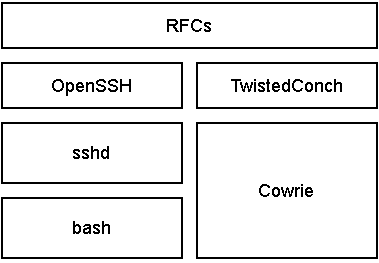
\includegraphics{figures/cowrie-openssh.pdf}
    \caption[Architecture of OpenSSH and Cowrie (derived from \cite{vetterl2020})]{Architecture of OpenSSH and Cowrie. OpenSSH and TwistedConch have subtle differences (derived from \cite{vetterl2020})}
    \label{fig:cowrie-openssh}
\end{figure}

\citet{vetterl2020} states that current low- and medium-interaction honeypots have a generic weakness due to the underlying off-the-shelf libraries.
Cowrie is based on TwistedConch, a Python 2/3 library that implements the SSH protocol.
Any bash command and its response are tweaked by Cowrie, and thus, resulting in a discrepancy to OpenSSH.
For example, Cowrie version $1.1.0$ missed \verb|tftp|\footnote{Is } and came with version $1.2.0$.
Therefore, it is a continuous struggle of adding new commands to avoid early disclosures of Cowrie.

\autoref{fig:cowrie-openssh} shows the difference between OpenSSH and Cowrie.
Both have to fulfill the RFC 4250 \cite{rfc4250} requirement on top.
OpenSSH and TwistedConch implement the SSH protocol.
As an example, \citet{vetterl2020} found that Cowrie used to have random bytes for the \verb|SSH2_MSG_KEXINIT| packet\footnote{Each packet consists of the packet and padding length, the \ac{mac}, a payload, and a random padding.} unlike OpenSSH.
With respect to RFC4253 \cite{rfc4253} that defines the \ac{bpp} of SSH, the random padding is used to solidify the total length of the packet to be a multiple of the cipher block size.
The RFC in section 6 defines that the padding have to consist of 4 random bytes.
Based on the statement of the OpenSSH authors, random bytes have been changed to \verb|NULL| characters due to no security implications.
Thus, an adversary could have detected a Cowrie honeypot with a single \verb|SSH2_MSG_KEXINIT| packet.
Nowadays, Cowrie adapted itself to have \verb|NULL| characters as padding.
However, these subtle differences influence the cosine similarity coefficient.

\begin{table}
    \caption{Overview of the cosine similarity of OpenSSH, Cowrie, and Twisted.}
    \begin{tabular}{lc|cccccccccc}
    \toprule
                   &   & A & B      & C      & D      & E      & F      & G      & H      & I      & J      \\
    \hline
    OpenSSH 6.6    & A & - & $0.98$ & $0.98$ & $0.94$ & $0.94$ & $0.42$ & $0.78$ & $0.79$ & $0.79$ & $0.79$ \\
    OpenSSH 6.7    & B &   & -      & $0.98$ & $0.98$ & $0.98$ & $0.41$ & $0.80$ & $0.81$ & $0.81$ & $0.80$ \\
    OpenSSH 6.8    & C &   &        & -      & $0.96$ & $0.96$ & $0.42$ & $0.78$ & $0.79$ & $0.79$ & $0.79$ \\
    OpenSSH 7.2    & D &   &        &        & -      & $0.98$ & $0.42$ & $0.80$ & $0.80$ & $0.80$ & $0.80$ \\
    OpenSSH 7.5    & E &   &        &        &        & -      & $0.42$ & $0.78$ & $0.79$ & $0.79$ & $0.79$ \\
    \\
    \cline{1-2} \cline{8-12}
    \\
    Twisted 15.2.1 & F &   &        &        &        &        & -      & $0.50$ & $0.51$ & $0.51$ & $0.52$ \\
    \\
    \cline{1-2} \cline{9-12}
    \\
    Cowrie 96ca2ba & G &   &        &        &        &        &        & -      & $0.98$ & $0.98$ & $0.98$ \\
    Cowrie dc45961 & H &   &        &        &        &        &        &        & -      & $0.99$ & $0.99$ \\
    Cowrie dbe88ed & I &   &        &        &        &        &        &        &        & -      & $0.99$ \\
    Cowrie fd801d1 & J &   &        &        &        &        &        &        &        &        & -      \\
    \bottomrule
    \end{tabular}
    \label{tab:cosine-similarity}
\end{table}

\section{Disguising Cowrie}

Cowrie has to be tweaked to hide its generic weakness.
Fixing the major flaws in Cowrie to avoid early detection remains an ephemeral patch.
Therefore, a new solution is required to disguise Cowrie.
Otherwise, adversaries would blacklist any related host machine returning a similar cosine similarity coefficient.
\citet{vetterl2020} suggested the solution to use OpenSSH as an intermediary instance between the attacker and Cowrie. 
OpenSSH itself is not capable by default of proxying commands, therefore, we have to adjust the latest OpenSSH version to enable this feature.
\autoref{fig:cowrie-fix} visualizes our idea.
Cowrie is hidden in the background, and is only accessible through the loopback address \ipAddress{127.0.0.1:640522}.
Our updated SSH version \verb|sshd| is exposed to the Internet, and is accessible through \ipAddress{129.206.5.157:2222}.
Any connection obtain to OpenSSH will be forwarded to our honeypot.
Respectively, our attacker should not be able to detect Cowrie by response deviations because any response packet runs through OpenSSH.

\begin{figure}[ht]
    \centering
    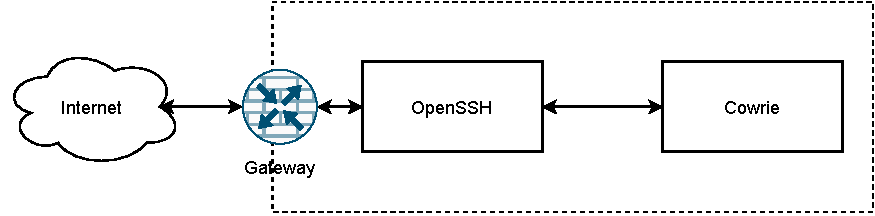
\includegraphics{figures/sshd-honeypot.pdf}
    \caption[Architecture of OpenSSH and Cowrie (derived from \cite{vetterl2020})]{Architecture of OpenSSH and Cowrie. OpenSSH and TwistedConch have subtle differences (derived from \cite{vetterl2020})}
    \label{fig:cowrie-fix}
\end{figure}

Forwarding SSH packets between OpenSSH and Cowrie would result in blocking any fingerprinting activities.


\section{Experiment}

Our experiment exists out of two steps.
First, we want to reproduce the cosine similarity coefficient that \citet{vetterl2020} claims.
Second, we want to disguise Cowrie with the idea we have mentioned beforehand.

Most challenging is the reproduction of the outdated OpenSSH library that \citet{vetterl2020} refers to.
In his work he used OpenSSH $7.3P1$ which deviates from the latest version $8.8P1$.
For the \verb|SSH2_MSG_KEXINIT| packet, the encryption algorithm blowfish-cbc and host key algorithm has been removed with version $7.6P1$, and thus, are outdated.
Building the version $7.3P1$ requires the libraries libssl (1.0.2), libssl-dev (1.0), libssh-dev (0.7.3-2), and libssh-4 (0.9.6-1).
Using the latest versions of these libraries result in errors such as missing encryption algorithms.
After compiling the package, we test its behavior with a Debian 11 Buster and a Debian Jessie 9 Docker image.
Both are new machines that have no other packages installed than the OpenSSH server.
Debian 11 uses the latest OpenSSH version whereas Jessie is at $6.7P1$.
These environments help us to uniquely identify variations in the protocol version.

\begin{figure}
    \lstinputlisting[language=bash, caption={OpenSSH connection attempt with probed SSH packet}, label={lst:ssh-openssh}]{listings/ssh-openssh.txt}
\end{figure}

\autoref{lst:ssh-openssh} shows the connection attempt with our adjusted version string and \verb|SSH2_MSG_KEXINIT| packet.
Using the outdated OpenSSH version $7.3P1$ results in an incompatibility.
OpenSSH outlines that blowfish-cbc is not supported anymore and remains usable for compatibility for the client until $7.6P1$.
However, we found out that patches removed the blowfish-cbc for the SSH daemon, and thus, a reproduction is feasible.
Moreover, \citet{vetterl2020} does not outline any expected response of OpenSSH, we can just assume that a connection attempt would have been successful due to the existing cipher during that time.
Adapting OpenSSH version $8.8P1$ with chacha20-poly1305 instead of blowfish-cbc results in a successful connection attempt.
Therefore, we have adapted the key exchange initialization to use chacha20-poly1305 instead.

\begin{figure}
    \lstinputlisting[language=bash, caption={Cowrie connection attempt with probed SSH packet}, label={lst:ssh-cowrie}]{listings/ssh-cowrie.txt}
\end{figure}

Most interesting question remains the response deviation of Cowrie.
Therefore, we use the default Cowrie implementation of our T-Pot deployment.
Currently, it uses Cowrie $v.2.3.0$.
\autoref{lst:ssh-cowrie} outlines the connection attempt of Cowrie.
Unambiguously, Cowrie results in a bad packet length, and thus, deviates fundamentally from OpenSSH.
Any adversary who modifies its SSH client could catch the exception and stop any further attacks.
We found out that the version string causes this error.
The library TwistedConch throws this exception. % TODO Debug Cowrie

\begin{figure}
    \lstinputlisting[language=bash, caption={Disguised Cowrie connection attempt with probed SSH packet}, label={lst:ssh-cowrie-fixed}]{listings/ssh-cowrie-fixed.txt}
\end{figure}

The next step is to disguise Cowrie behind an OpenSSH server.
As we have seen beforehand, the OpenSSH server should work as an intermediary between Cowrie and the attacker.
We have implemented this concept in heiCLOUD.
